\documentclass[11pt,class=report,crop=false]{standalone}
\usepackage[screen]{../python}

\begin{document}


%====================================================================
\chapitre{Physique quantique}
%====================================================================

\insertvideo{e5K5bN2H8Mw}{partie 6.1. Particule}

\insertvideo{5wTVAvC6q8U}{partie 6.2. Dualité onde/corpuscule}

\insertvideo{hy_C1vnKeg0}{partie 6.3. Fonction d'onde et équation de Schrödinger}

\insertvideo{h3T3swzS1dw}{partie 6.4. Qubits}



\objectifs{L'objectif est de comprendre les notions de base de la physique quantique.}

%%%%%%%%%%%%%%%%%%%%%%%%%%%%%%%%%%%%%%%%%%%%%%%%%%%%%%%%%%%%%%%%%%%%%
\section{Particule}

%--------------------------------------------------------------------
\subsection{Bestiaire}

Commençons par un tour d'horizon des particules :
\begin{itemize}
  \item Les \defi{protons} (charge électrique positive) et les \defi{neutrons} (pas de charge) constituent le noyau des atomes.

  \item Autour du noyau gravitent des \defi{électrons} (charge négative). 

  \item Un modèle simple de structure de l'atome est décrit par les électrons qui se répartissent sur des couches sphériques ayant pour centre le noyau, ce modèle est maintenant désuet. Avec la mécanique quantique, on considère qu'un électron peut être à n'importe quelle position  autour du noyau, mais pas partout avec la même probabilité.

\myfigure{0.5}{
\tikzinput{fig-physique-01}\qquad\qquad
\tikzinput{fig-physique-02}
}

  \item Le \defi{photon} est la particule fondamentale de la lumière (et des ondes électromagnétiques). Il n'a ni masse ni charge.
\end{itemize}


%--------------------------------------------------------------------
\subsection{Quantification}

Des expériences montrent que le changement d'état des électrons dans un atome correspond à des niveaux d'énergie bien déterminés.
On le conçoit bien avec le modèle dans lequel les électrons gravitent sur des couches : pour qu'un électron passe à une couche supérieure, il faut lui fournir un certain niveau d'énergie.

\myfigure{0.5}{
\tikzinput{fig-physique-03}
}

La formule qui calcule l'énergie à fournir est donnée par :
\mybox{$\Delta E = E_{\text{après}} - E_{\text{avant}} = n h \nu$}
où $n$ est un entier, $\nu$ est la fréquence du rayonnement reçu (ou émis) (exprimée en $s^{-1}$)
et $h$ est la \defi{constante de Planck}\index{constante de Planck}, $h \simeq 6.62 \cdot 10^{-34} \, J\cdot s$.

Il y a donc un phénomène de \defi{quantification}, car l'énergie reçue (ou émise) ne peut prendre que des valeurs discrètes, c'est-à-dire que l'on peut indexer par l'entier $n$ qui vaut $1$, $2$, $3$\ldots{}  et non par des valeurs continues (comme on l'aurait avec un paramètre réel $t \ge 0$).

La \defi{formule de Bohr-Einstein} lie l'énergie à la fréquence :
\mybox{$E = h \nu$}


On rencontre aussi souvent la \defi{constante de Planck réduite}:
\mybox{$\displaystyle \hbar = \frac{h}{2\pi}$}

%--------------------------------------------------------------------
\subsection{Principe d'incertitude d'Heisenberg}

Le \defi{principe d'incertitude d'Heisenberg}\index{principe d'incertitude d'Heisenberg} s'énonce mathématiquement ainsi:
\mybox{$\displaystyle \sigma_{\mathbf x}\cdot\sigma_{\mathbf v} \ge \frac{h}{4\pi m}$}
où :
\begin{itemize}
    \item $\sigma_{\mathbf x}$ est l'écart-type d'une série de mesures de la position $\mathbf x = (x,y,z)$ d'une particule. Cet écart-type est obtenu en répétant plusieurs fois l'expérience suivante : on prépare la particule, toujours avec le même état initial, puis on mesure sa position.
    
    \item $\sigma_{\mathbf v}$ est l'écart-type de la mesure de la vitesse de la particule $\mathbf v = (v_x,v_y,v_z)$.
\end{itemize}

L'interprétation de la formule est la suivante : si on connaît avec une grande précision la position d'une particule alors on ne peut pas connaître très précisément sa vitesse. Et réciproquement si on connaît très précisément la vitesse, on ne peut pas connaître très précisément la position. 

En effet, imaginons que l'on connaisse très précisément la position d'une particule,
alors lorsque l'on va répéter la mesure de la position, on obtiendra presque toujours la même mesure. Autrement dit, les écarts entre les différentes mesures sont tout petits : $\sigma_{\mathbf x} \simeq 0$. Par le principe d'incertitude,
$\sigma_{\mathbf v} \ge \frac{h}{4\pi m\sigma_{\mathbf x}}$
doit être très grand. C'est-à-dire que les différentes mesures de la vitesse conduisent à des grands écarts.

L'incertitude est d'autant plus grande que la masse $m$ est petite. Par contre la constante de Planck $h$ étant toute petite ($h \simeq 6.62 \cdot 10^{-34} \, J\cdot s$), cette incertitude ne concerne vraiment que les particules et pas les objets plus gros de la physique classique.


%%%%%%%%%%%%%%%%%%%%%%%%%%%%%%%%%%%%%%%%%%%%%%%%%%%%%%%%%%%%%%%%%%%%%
\section{Dualité onde/corpuscule}

\index{dualite onde corpuscule@dualité onde/corpuscule}

En physique classique, on sépare l'étude des corpuscules (un objet matériel comme une bille) de celle des ondes (par exemple une onde sonore ou bien la lumière). En physique quantique, une particule se comporte à la fois comme une onde et un corpuscule. C'est la très déroutante \og{}dualité onde/corpuscule\fg{}.

\textbf{Corpuscule.} 
Un \og{}corpuscule\fg{} est un petit objet aux propriétés physiques bien déterminées : comme sa position $(x,y,z)$, sa vitesse $(v_x,v_y,v_z)$, sa masse\ldots{} Il peut avoir une taille mais est souvent modélisé par un point.
La mécanique d'un point matériel est bien connue, même si on a vu, avec le principe d'incertitude d'Heisenberg, que la mesure de la position et celle de la vitesse ne sont pas si évidentes que cela !

\myfigure{0.5}{
\tikzinput{fig-physique-08}
}

\textbf{Onde.}
Une \og{}onde\fg{} est la variation d'une propriété physique par propagation. Par exemple, une onde sonore est la variation de la pression : un mouvement initial fait que des molécules d'air viennent frapper les molécules voisines qui à leur tour déplacent les molécules suivantes. Pourtant chaque molécule ne se déplace presque pas (elle revient à sa place après avoir rebondi sur sa voisine) par contre l'onde se déplace.
Une vague est un autre exemple d'onde, les molécules d'eau font varier la hauteur. Pourtant les molécules d'eau ne se déplacent pas en suivant les vagues. D'ailleurs un bouchon flottant sur les vagues ne se déplace pas horizontalement.

Les ondes électromagnétiques se déplacent dans le vide à la vitesse de la lumière ($300\,000$ $km \cdot s^{-1}$). Le courant électrique se déplace dans un fil de cuivre un peu moins vite ($200\,000$ $km \cdot s^{-1}$). Par contre les électrons qui propagent ce courant se déplacent très lentement (quelques centimètres par heure).


\bigskip

Voici deux vues d'une onde sinusoïdale : la première vue en une vue en coupe (on voit les vagues avec les crêtes et les creux), la seconde vue est une vue de dessus, comme si on avait jeté un caillou dans l'eau et qu'on observe les lignes de crête circulaires.

\myfigure{0.5}{
\tikzinput{fig-physique-10}
}


Une des propriétés fondamentales des ondes est le principe de superposition.
Deux ondes se superposent (figure de gauche), ce qui peut conduire à une onde renforcée (figure centrale), ou bien à annulation (figure de droite).

\myfigure{0.45}{
\tikzinput{fig-physique-09a}
\tikzinput{fig-physique-09b}
\tikzinput{fig-physique-09c}
}


Nous allons étudier les phénomènes d'interférence à l'aide de l'expérience de Young à deux fentes, mais commençons par un cas plus simple.

\textbf{Expérience à une fente.}
Une onde est émise d'un point. Elle se propage vers une paroi opaque dans laquelle on a effectué une fente mince (ou bien un petit trou). En passant cette fente l'onde se diffracte (elle perd sa direction d'origine) et vient éclairer un écran récepteur.
Que voit-on sur cet écran ? L'onde frappe l'écran de manière essentiellement uniforme. En réalité la partie centrale est plus touchée que les bords et fait apparaître une large bande de diffraction, mais ce n'est pas important pour nous.

Ci-dessous le résultat d'une expérience à une fente à l'aide d'une lumière laser.
\begin{center}
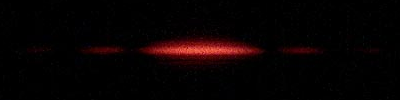
\includegraphics[scale=\myscale,scale=0.9]{figures/fig-une-fente}
\end{center}


\myfigure{0.5}{
\tikzinput{fig-physique-11}
}


\textbf{Expérience à deux fentes.}

On reprend l'expérience mais cette fois avec deux fentes.

\myfigure{0.5}{
\tikzinput{fig-physique-13}
}

 L'onde passe simultanément par les deux trous et se diffracte. Un point de l'écran est donc atteint depuis deux sources différentes. Que voit-on sur l'écran ? On note des franges minces et nettes qui sont des franges d'interférence. 

\begin{center}
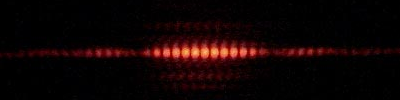
\includegraphics[scale=\myscale,scale=0.9]{figures/fig-deux-fentes}
\end{center}

Comment expliquer cela ? Plaçons-nous en un point $P$ de l'écran. Ce point capte l'onde depuis deux sources différentes $F_1$ et $F_2$, mais ces deux sources ne sont pas situées à la même distance de $P$ : $PF_1 \neq PF_2$. Il y a donc un décalage (appelé déphasage) entre l'onde reçue depuis $F_1$ et l'onde reçue depuis $F_2$. Selon la position du point $P$, les ondes peuvent s'amplifier ce qui conduit aux franges claires les plus atteintes.
C'est ce qu'il se passe ci-dessous au point $P$ où les deux sinusoïdes arrivent en phase (les deux crêtes arrivent en même temps au point $P$, et au fil du temps les ondes restent en phase).

\myfigure{0.5}{
\tikzinput{fig-physique-12a}
}

Mais les ondes peuvent s'annuler ce qui correspond aux franges sombres (rien n'est capté). C'est le cas au point de la configuration ci-dessous. En ce nouveau point $P$ une sinusoïde  présente une crête alors que l'autre sinusoïde est à un creux (de même amplitude), la résultante des deux est nulle (et reste nulle au fil du temps).


\myfigure{0.5}{
\tikzinput{fig-physique-12b}
}

Mathématiquement si le signal issu de $F_1$ est $f_1(t) = \sin(\omega t)$
alors le signal issu de $F_2$ est $f_2(t) = \sin(\omega t + \phi_P)$ où $\phi_P$ est le \defi{déphasage}, sa valeur dépend de la position du point $P$.
Si $\phi_P$ est de la forme $2k\pi$ alors $f_2(t) = \sin(\omega t)$ et donc les ondes s'ajoutent pour donner $f(t) = f_1(t)+f_2(t) = 2\sin(\omega t)$.
Par contre si $\phi_P$ est de la forme $\pi + 2k\pi$ alors $f_2(t) = -\sin(\omega t)$ et donc les ondes s'annulent pour donner $f(t) = f_1(t)+f_2(t) = 0$.


\bigskip

Que se passe-t-il si on réalise l'expérience à deux fentes avec un corpuscule (par exemple en envoyant une multitude de petites billes) au lieu d'une onde ? Chaque corpuscule passe par la fente 1 ou bien par la fente 2 (mais pas les deux) et il y a un phénomène de diffraction à chaque fente. Que voit-on à l'écran ? L'écran est uniformément atteint. Il n'y a pas de phénomène d'interférence puisque une bille ne passe que par un seul trou.


\textbf{Expérience quantique à deux fentes.}
Voici l'expérience incroyable : on envoie une à une des particules à travers le dispositif à deux fentes. Ces particules sont par exemple des photons ou des électrons.
Voici ce que l'on obtient à l'écran au fur et à mesure des lancers (ici des électrons).
Nombre d'électrons captés (a) 11 ; (b) 200, (c) 6000, (d) 40\,000, (e) 140\,000.

\begin{center}
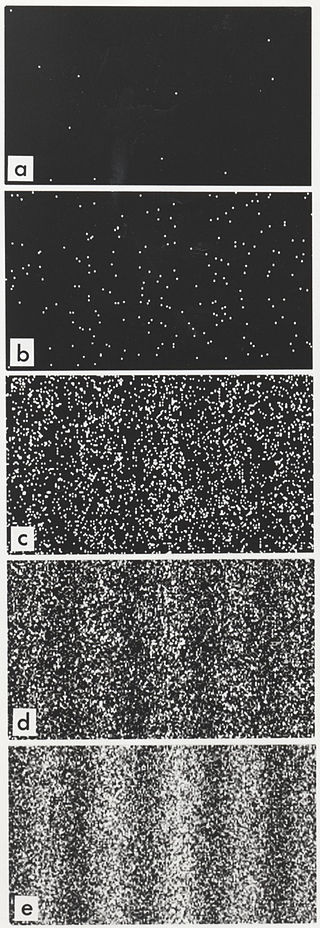
\includegraphics[scale=\myscale,scale=1.2]{figures/fig-interferences}
\end{center}


On observe des franges d'interférence alors qu'on a envoyé les particules une par une !
Ces particules sont bien des corpuscules puisque qu'on les envoie une par une et on peut même les compter. Mais les franges d'interférence prouvent que ces particules sont aussi des ondes ! Ainsi on ne peut parler de trajectoire pour une particule quantique. Une particule quantique possède à la fois des propriétés corpusculaires et des propriétés ondulatoires : c'est la \og{}dualité onde/corpuscule\fg{}.

\bigskip

\textbf{Mesure.} 
Si on reprend l'expérience quantique à deux fentes mais que cette fois on mesure par quel trou la particule passe, alors on obtient un écran uniformément atteint !
Il faut comprendre que la mesure perturbe irrémédiablement l'état quantique et la particule perd ses caractéristiques quantiques. Le fait de rajouter une mesure entraîne que ce n'est pas du tout la même expérience qu'auparavant.


\bigskip

\textbf{Le chat de Schrödinger.}
\index{chat de Schordinger@chat de Schrödinger}
Dans le monde dans lequel nous vivons les objets sont \og{}gros\fg{} et leur appliquer des propriétés quantiques n'a pas trop de sens. C'est pourtant ce que l'on fait avec l'expérience de pensée du chat de Schrödinger. Dans une boîte recouverte d'un voile noir, on met un chat, un fiole de poison et une particule. 
Si la particule se désintègre, elle casse la fiole qui libère le poison et le chat meurt.


\myfigure{1}{
\tikzinput{fig-physique-14}
}

La particule a une demi-vie d'une heure, c'est-à-dire qu'au bout d'une heure, il y a une chance sur deux qu'elle se soit désintégrée. 
Question : au bout d'une heure le chat est-il mort ou vivant ? Ou bien moitié-mort et moitié-vivant ? 
% Et qui tue le chat ? 
% N'est-ce pas vous lorsque vous lever le voile ? 
En fait, tant que le voile noir n'est pas levé le chat n'est pas vraiment mort. Par contre lever le voile (ce qui correspond à une mesure) enlève le caractère mi-mort/mi-vivant au chat et rend l'état du chat certain.
C'est assez perturbant ! 

On retient que la mécanique quantique est une théorie qui s'applique aux particules de petite taille, et souvent sur de courtes périodes.



%%%%%%%%%%%%%%%%%%%%%%%%%%%%%%%%%%%%%%%%%%%%%%%%%%%%%%%%%%%%%%%%%%%%%
\section{Fonction d'onde et équation de Schrödinger}

%--------------------------------------------------------------------
\subsection{Fonction d'onde}

\textbf{Fonction d'onde.}
Le mouvement d'une particule en physique classique est décrit par sa position $(x,y,z)$ (qui peut varier en fonction du temps) et sa vitesse $(v_x,v_y,v_z)$. Ce modèle n'est plus valide en physique quantique.

En physique quantique on associe à une particule une \defi{fonction d'onde}\index{fonction d'onde} $\Psi$ :
$$\Psi(x,y,z,t) : \Rr^4 \longrightarrow \Cc.$$
Cette fonction dépend du point de l'espace $(x,y,z)$ et du temps $t$ ; elle est à valeurs complexes et n'a pas d'interprétation physique.

\bigskip

\textbf{Probabilité.}
Par contre la fonction d'onde permet de déterminer la probabilité de la particule d'être à une position donnée : la probabilité que la particule soit mesurée à la position $(x,y,z)$ au temps $t$ est donnée par la densité de probabilité :
$$\left| \Psi(x,y,z,t) \right|^2.$$
Autrement dit :
$$\dd P(x,y,z,t) = \left| \Psi(x,y,z,t) \right|^2 \dd x \dd y \dd z$$
où $\dd x \dd y \dd z$ représente un petit cube élémentaire autour de la position $(x,y,z)$.
Nous avons la relation :
$$\int \left| \Psi(x,y,z,t) \right|^2 \dd x \dd y \dd z = 1$$
qui signifie que la somme des probabilités (pour toutes les positions possibles) est $1$.

\bigskip

\textbf{Mesure de la position.}
Il faut bien comprendre que l'on ne connaît pas la position de la particule. Ce n'est pas un défaut ou un manque de précision mais la base de la mécanique quantique. 
La notion de position n'a pas de sens avant la mesure. On pourrait dire que la particule est \og{}partout\fg{}, et que c'est la mesure qui détermine une position $(x,y,z)$. 
Enfin, même si la particule peut être mesurée à n'importe quelle position, certaines positions sont cependant plus probables que d'autres.

Voici un exemple de répartition des mesures d'une position $x$ (on se limite à la mesure de la seule coordonnée $x$) obtenue en répétant l'expérience : je prépare la particule, puis je mesure la position $x$. On note que certaines positions sont plus fréquentes que d'autres.

\myfigure{1}{
\tikzinput{fig-physique-04}
}

Mathématiquement les résultats s'interprètent avec la densité de probabilité $P(x) = \left| \Psi(x) \right|^2$ qui décrit la répartition probable. L'aire sous la courbe vaut $1$, car $\int \left| \Psi(x) \right|^2 \dd x = 1$ (ce qui est la traduction que la somme des probabilités vaut $1$).

\myfigure{1}{
\tikzinput{fig-physique-05}
}


%--------------------------------------------------------------------
\subsection{Équation de Schrödinger}

La loi qui régit le mouvement d'une particule classique est le principe fondamental de la mécanique :
$$\sum \vec F = m \vec a.$$
La somme des forces est égale à la masse multipliée par l'accélération.
L'accélération est la dérivée de la vitesse par rapport au temps, qui elle-même est la dérivée de la position par rapport au temps.
Ainsi on n'obtient pas exactement la position $\mathbf{x} = (x(t),y(t),z(t))$  mais une équation différentielle faisant intervenir la dérivée seconde $\frac{\dd^2 \mathbf x}{\dd t^2}(t)$. Si on sait résoudre cette équation différentielle (ce qui n'est pas toujours possible), on trouve la position $\mathbf{x}$.

\bigskip

Qu'en est-il pour la mécanique quantique ?
On a vu que le comportement d'une particule est régi par sa fonction d'onde $\Psi(x,y,z,t)$.
La loi quantique fondamentale qui régit le comportement d'une particule libre est donnée par \defi{l'équation de Schrödinger}\index{equation de Schodinger@équation de Schrödinger} :
\mybox{$\displaystyle \ii \frac{\partial \Psi}{\partial t} = - \frac{\hbar}{2m} \Delta \Psi$}
où :
\begin{itemize}
  \item $\ii$ est le nombre complexe avec $\ii^2 = -1$,
  \item $\hbar = \frac{h}{2\pi}$ est la constante de Planck réduite,
  \item $m$ est la masse de la particule,
  \item $\Psi(x,y,z,t)$ est la fonction d'onde,
  \item $\frac{\partial \Psi}{\partial t}$ est la dérivée de la fonction d'onde par rapport au temps (on parle de dérivée partielle par rapport à $t$),
  \item $\Delta \Psi$ est le Laplacien de $\Psi$, c'est la somme des dérivées partielles secondes en $x$, $y$ et $z$ :
$$\Delta \Psi = \frac{\partial^2 \Psi}{\partial x^2} + \frac{\partial^2 \Psi}{\partial y^2} + \frac{\partial^2 \Psi}{\partial z^2}.$$
\end{itemize}

L'équation de Schrödinger est une équation différentielle (ici une équation aux dérivées partielles) qui régit $\Psi$ et donc le comportement de la particule. Par contre, en trouver des solutions est difficile.
Si de plus la particule est soumise à des forces externes, données par un potentiel $V(x,y,z,t)$, alors l'équation de Schrödinger devient :
$$\ii \hbar \frac{\partial \Psi}{\partial t}(x,y,z,t) = - \frac{\hbar^2}{2m} \Delta \Psi(x,y,z,t) + V(x,y,z,t)\Psi(x,y,z,t).$$

%--------------------------------------------------------------------
\subsection{Principe de superposition}

\index{superposition}

Il est facile de vérifier que si $\Psi_1$ et $\Psi_2$ sont deux fonctions d'onde, solutions de l'équation de Schrödinger alors la combinaison linéaire 
$$\Psi = \alpha \Psi_1 + \beta \Psi_2 \qquad \text{ avec } \alpha, \beta \in \Cc$$ est aussi une solution (il faut tout de même vérifier la condition de normalisation $\int |\Psi|^2 = 1$).

Par contre en termes de probabilités, c'est plus compliqué. Si on note $P_1 = |\Psi_1|^2$ et $P_2 = |\Psi_2|^2$ les densités de probabilité associées aux deux fonctions d'onde et avec par exemple $\Psi = \frac{1}{\sqrt2} (\Psi_1+\Psi_2)$, 
alors on pourrait penser que la densité de probabilité $P = |\Psi|^2$ est $\frac12(P_1+P_2)$ mais ce n'est pas le cas. En effet :
\begin{align*}
P &= |\Psi|^2 = |\Psi_1+\Psi_2|^2 = \frac12(\Psi_1+\Psi_2)(\Psi_1+\Psi_2)^* \\
&= \frac12(|\Psi_1|^2+|\Psi_2|^2 + \Psi_1\Psi_2^* + \Psi_1^*\Psi_2)
= \frac12(P_1+P_2 + \Psi_1\Psi_2^* + \Psi_1^*\Psi_2).
\end{align*}

Le terme $\Psi_1\Psi_2^* + \Psi_1^*\Psi_2$ est un terme d'interférence entre les deux fonctions d'ondes.


%%%%%%%%%%%%%%%%%%%%%%%%%%%%%%%%%%%%%%%%%%%%%%%%%%%%%%%%%%%%%%%%%%%%%
\section{Qubits}

%--------------------------------------------------------------------
\subsection{Réalisation de qubits}

\index{qubit!realisation@réalisation}

Il existe de nombreuses façons de réaliser physiquement un qubit, chacune présentant ses avantages et ses défis technologiques. Il est encore difficile de déterminer laquelle de ces technologies permettra de construire l'ordinateur quantique du futur. 

\begin{itemize}

  \item Polarisation des photons. La lumière polarisée vibre simultanément dans deux directions orthogonales. La mesure peut conduire à la polarisation horizontale $\rightarrow$ (qui est $\ket0$) ou verticale $\uparrow$ (qui est $\ket1$).

  \item Spin d'électrons piégés. Les électrons possèdent un mouvement cinétique interne. On dit qu'un électron \og{}tourne sur lui-même\fg{}. Le moment cinétique peut prendre une infinité de valeurs. Mais lorsque l'on mesure ce moment cinétique on n'obtient que deux valeurs possibles $+\frac\hbar2$ ou $-\frac\hbar2$.
  On note $\ket0$ et $\ket1$ ces deux mesures possibles. 
  Par contre avant la mesure, le moment cinétique avait la forme d'un qubit
  $\ket\psi = \alpha\ket0+\beta\ket1$ avec $|\alpha|^2+|\beta|^2=1$.
 
  \item Ions piégés. Les ions d'atomes sont piégés dans une cavité magnétique et dans le vide, ils sont manipulés par des rayons laser.
  
  \item Atomes froids. Des atomes sont refroidis par des lasers, leur état quantique correspond à leur niveau d'énergie, ils sont également manipulés par des lasers.
  
  \item Les supra-conducteurs sur silicium. L'objet quantique est dans ce cas un courant obtenu dans une jonction Josephson constituée par des oxydes d'aluminium sur des puces de silicium. L'état de ces qubits est manipulé par des impulsions à micro-onde qui constituent les portes quantiques.
  
  % \item D'autres dispositifs existent ou sont à l'étude, par exemple à l'aide de centres NV, (Nitrogen Vacancy) dans du carbone diamant), ou encore dans le futur peut-être avec des fermions de Majorana.
  
\end{itemize}

%--------------------------------------------------------------------
\subsection{Mesure}


\index{qubit!mesure}

La mesure joue un rôle important en physique quantique : la mesure est un acte irréversible qui change la fonction d'onde.
Avant la mesure, la fonction d'onde d'une particule peut conduire à plusieurs mesures possibles (si on répète l'expérience de la préparation de la particule, puis de la mesure, on obtient des résultats qui peuvent être différents à chaque mesure).
Par contre après une mesure, la fonction d'onde est changée définitivement, on parle de la \og{}réduction du paquet d'onde\fg{}, et ne conduit plus qu'à un seul résultat : si on effectue une seconde mesure immédiatement après, on obtient le même résultat.

La théorie de la décohérence quantique tente d'expliquer le passage du monde quantique à la physique classique.
Un état quantique ne reste \og{}cohérent\fg{} que s'il n'est pas perturbé. Une particule vit dans un environnement complexe et perd sa cohérence quantique plus ou moins rapidement. En particulier une mesure physique vient déranger la cohérence, et la particule change d'état quantique.
Par exemple une molécule (de taille environ $10^{-7}$ m) dans un vide de laboratoire conserve sa cohérence quantique seulement environ $10^{-17}$ seconde.


%--------------------------------------------------------------------
\subsection{Intrication quantique}

\index{intrication quantique}

\textbf{Analogie élémentaire.}
Commençons par des analogies simplistes. On dispose de deux cartes : une rouge et une bleue. On place ces deux cartes dans deux enveloppes. On donne, au hasard, une enveloppe à Alice et une autre à Bob. Ensuite Alice et Bob se séparent. Pour Alice la probabilité d'avoir la carte rouge est de $1/2$, la carte bleue également $1/2$. De même pour Bob. Si Alice ouvre son enveloppe, et par exemple découvre la carte rouge. Alors bien sûr, elle a la carte rouge avec probabilité $1$, mais surtout Bob a maintenant la carte bleue avec probabilité $1$, même s'il n'a pas ouvert son enveloppe.
Les deux cartes sont liées : on parle d'intrication. La mesure de l'un fait disparaître les probabilités pour les deux cartes.

\myfigure{0.5}{
\tikzinput{fig-physique-06}
}
 
Un des principes de la théorie de la relativité est qu'aucune particule, aucun signal, aucune information ne peut voyager plus vite que la lumière. Ce principe est-il violé ici ? Dès qu'Alice découvre que son enveloppe contient la carte rouge, elle a automatiquement la certitude que Bob a en sa possession la carte bleue. Ce n'est pas un paradoxe car en fait Bob reste ignorant de la couleur de sa carte. Il peut toutefois connaître la couleur de sa carte sans ouvrir son enveloppe. Il suffit qu'Alice lui téléphone et lui dise qu'elle a eu la carte rouge, ainsi Bob saura qu'il a la carte bleue. Mais aucun principe n'est violé car la vitesse de transmission téléphonique d'une information ne dépasse pas la vitesse de la lumière.

\bigskip 
\textbf{Autre analogie.} On continue avec une expérience un peu plus physique.
On prend deux particules identiques que l'on fait cogner l'une contre l'autre au point $O$.
L'une part vers Alice et l'autre vers Bob. Elles ont exactement des mouvements opposés : position et vitesse sont égales au signe près. Si Alice mesure la position ou la vitesse de sa particule, alors cela détermine la position ou la vitesse de la particule Bob. Ainsi Bob peut connaître la position ou la vitesse de sa particule sans faire lui-même une mesure.

\myfigure{0.5}{
\tikzinput{fig-physique-07}
}

\bigskip
\textbf{Expérience réelle.} Dans la pratique on sait préparer deux photons qui sont intriqués par polarisation. Ensuite on sait envoyer les photons à des centaines de kilomètres l'un de l'autre en les maintenant intriqués, ce qui permet de réaliser le codage super-dense et la téléportation quantique.

\bigskip
\bigskip

\emph{Crédits photos.} \href{https://en.wikipedia.org/wiki/Double-slit_experiment}{Wikipedia, \emph{Double-slit experiment}} :
\begin{itemize}
  \item pour les photos de l'expérience en lumière laser à une et deux fentes, Jordgette, CC BY-SA 3.0,
  \item pour les photos de l'interférence quantique, Dr. Tonomura, CC BY-SA 3.0.
\end{itemize}



\end{document}
